
\chapter{Solvation Properties\label{chpt:solvation-properties}}

The solvation free energy and solvent structure are the most important
property that we seek; as shown in previous sections, they can be
both obtained by the minimization of the free energy functional $\mathcal{F}[\rho]$.
Here is a discussion about some corrections needed for charged solutes
and some profiles of structures deduced from the solvent density.

\section{Free energy correction for single ions\label{sec:Free-energy-correction}}

In the calculation of external potential as well as the total solvation
free energy, the use of different conventions can lead to a charge-independent
offset, which introduces error for charged solutes \citep{Kastenholz_2006_I,Kastenholz_2006_II,Hunenberger_book}.
This offset is mainly caused by two sources: (1) resulting from the
use of a finite system size; in our case, is a system with cubic periodic
boundary conditions, which presents artificial interactions between
the ion and its own periodic copies, as well as between the solvent
and the periodic copies of the ion (Type-B); (2) resulting from the
choice of convention for summing up the contributions of solvent charges
to the electrostatic potential in the sample system (Type-C).

\subsection{Correction of type B}

Type B correction should be added for systems with finite size or
periodic boundary conditions, accounting for the error in the solvent
polarization: \marginpar{Another way to evaluate this error is to make a numerical extrapolation
of the inverse of the box size $\left(1/L\right)$; it is more accurate,
but demands much more calculation.}
\begin{equation}
\Delta G_{B}=\frac{1}{8\pi\varepsilon_{0}}\left(1-\varepsilon^{-1}\right)\frac{q^{2}}{L}\left[\xi+\frac{4\pi}{3}\left(\frac{R_{\mathrm{I}}}{L}\right)^{2}-\frac{16\pi}{45}\left(\frac{R_{\mathrm{I}}}{L}\right)^{5}\right]\label{eq:corr-B}
\end{equation}
where

\begin{tabular}{cl}
 $\varepsilon_{0}$ & is the vacuum permittivity;\tabularnewline
$\varepsilon$ & is the solvent permittivity (dielectric constant), here $\varepsilon=71$
for water \citep{Kusalik_1994_dc_spc/e,SPC/E};\tabularnewline
$q$ & is the solute charge;\tabularnewline
$L$ & is the box length;\tabularnewline
$R_{\mathrm{I}}$ & is the ionic radius;\tabularnewline
$\xi$ & is the energy per particle in a simple cubic lattice, $\xi\simeq-2.837297$
\citep{nijboer}.\tabularnewline
 & \tabularnewline
\end{tabular} 

As $R_{\mathrm{I}}$ is significantly smaller than the size of the
computational box, i.e. $R_{\mathrm{I}}\ll L$, its quadratic as well
as higher order of $\left(R_{\mathrm{I}}/L\right)$ is considered
negligible, thus eq. (\ref{eq:corr-B}) becomes:
\begin{equation}
\Delta G_{\mathrm{B}}=\frac{\xi}{8\pi\varepsilon_{0}}\left(1-\varepsilon^{-1}\right)\frac{q^{2}}{L}
\end{equation}
which has the same form as the Born model in eq. (\ref{eq:born_model}).

\subsection{Correction of type C}

Type-C corrections are needed when the systems to be compared use
different electrostatic summation schemes: on the basis of point charges
within entire solvent molecules (M scheme) or on the basis of individual
point charges (P scheme), shown in figure \ref{fig:IQ-model-som-scheme}
(c) and (d), which brings a fixed free energy difference at the boundary.

\begin{figure}[h]
\begin{centering}
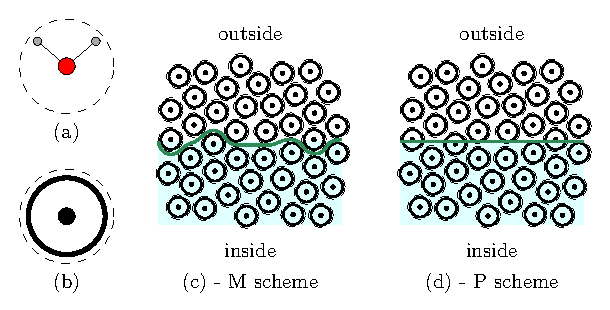
\includegraphics{_figure/ion_correction}
\par\end{centering}
\caption[IQ model and summation scheme]{IQ model and summation scheme. (a) The solvent molecule. (b) The
equivalent isotropic quadrupole (IQ) fluid model. (c) In the M scheme,
one evaluates the Coulombic potential generated by the solvent charges
belonging to all molecules within the boundary. (d) In the P scheme,
one evaluates the Coulombic potential generated by all solvent charges
within the boundary.\label{fig:IQ-model-som-scheme}}
\end{figure}

It can be deduced analytically by considering the solvent as a canonical
ensemble under the orientational disorder limit (ODL) \citep{Kastenholz_2006_I},
which becomes an isotropic quadrupole (IQ) fluid, whose solvent molecule
(figure \ref{fig:IQ-model-som-scheme} (b)) possesses the same quadrupole
trace \marginpar{$\gamma$ is elsewhere referred to as the spheropole moment \citep{Saunders_1992,Maschio_2012},
which is the spherical component of the quadrupole moment, and is
invariant with respect to rotations.}
\begin{equation}
\gamma=\mathrm{tr}(\mathbf{\mathcal{Q}})=\mathcal{Q}_{xx}+\mathcal{Q}_{yy}+\mathcal{Q}_{zz}
\end{equation}
where the quadrupole moment of the solvent molecule can be calculated
by its definition \citep{Multipole}
\begin{equation}
\mathcal{Q}_{ij}=\int_{V}r_{i}r_{j}\rho(\mathbf{r})\mathrm{d}v=\sum_{\alpha=1}^{N}q^{(\alpha)}r_{i}^{(\alpha)}r_{j}^{(\alpha)}
\end{equation}

It can be shown that the charge density of the solvent located within
the boundary of the sample system vanishes everywhere, except at the
boundary in the M scheme, which results in a uniform normal surface
polarization. The correction needed is:
\begin{equation}
\Delta G_{\mathrm{C}}=-q\left(1-\frac{4\pi R_{\mathrm{I}}^{3}}{3L^{3}}\right)\Delta\Phi_{\mathrm{ODL}}\label{eq:corr-C}
\end{equation}
where $\Delta\Phi_{\mathrm{ODL}}=\left(6\varepsilon_{0}\right)^{-1}\eta\gamma$,
$\eta$ being the solvent number density.

In the same way, when we consider $R_{\mathrm{I}}\ll L$, eq. (\ref{eq:corr-C})
becomes
\begin{equation}
\Delta G_{\mathrm{C}}=-\left(6\varepsilon_{0}\right)^{-1}\eta\gamma q
\end{equation}


\section{Solvation structure\label{sec:Solvation-structure}}

In MDFT, all the information about solvation structure can be deduced
from the solvent density $\rho(\mathbf{r},\mathbf{\Omega})$. Here
presents some examples of structure which are used in later chapters.

\subsection{Radial and site-site distribution function}

When the solvent is homogeneous, the \acs{PDF} can be reduced to
$g(r_{12})$, which is sometimes referred to as the radial distribution
function (\acs{RDF}). However, it can be also used as a key character
of the structure for inhomogeneous fluids, which can be calculated
equivalently as:
\begin{equation}
g(r)=\left\langle \rho(r,\hat{\mathbf{r}})\right\rangle =\dfrac{\int\rho(r,\hat{\mathbf{r}})\mathrm{d}s_{r}}{\int\mathrm{d}s_{r}}
\end{equation}

To do this integration, it is required to transform $\rho(\mathbf{r},\mathbf{\Omega})$
into spherical coordinates. But as $\rho(\mathbf{r},\mathbf{\Omega})$
in the code is a $N$-point discrete space grid:
\begin{equation}
\rho(\mathbf{r})=\int\mathrm{d}\mathbf{\Omega}\rho(\mathbf{r},\mathbf{\Omega})=\sum_{i=1}^{N}\rho_{i}\delta(\mathbf{r}-\mathbf{r}_{i})
\end{equation}
The best way to do the integration is to use a histogram approach.

The grid points are assumed to be homogenous in space, such that the
number of points entering in an arbitrary volume $v$ is proportional
to this volume. Obviously the grid of $\rho(\mathbf{r},\mathbf{\Omega})$
satisfies this assumption.

The average value of $g(r)$ between an interval $\delta r$ is
\begin{equation}
g(r_{i})=\left\langle g(r)\right\rangle _{r}^{r+\delta r}=\dfrac{\int_{r}^{r+\delta r}g(r)\mathrm{d}r}{\delta r}
\end{equation}

Thus
\begin{equation}
g(r_{i})=\dfrac{1}{\delta v_{i}}\int_{r}^{r+\delta r}\int_{s}\rho(r,\hat{\mathbf{r}})\mathrm{d}r\mathrm{d}s_{r}=\dfrac{1}{\delta v_{i}}\int_{v_{i}}\sum_{i=1}^{N}\rho_{i}\delta(\mathbf{r}-\mathbf{r}_{i})\mathrm{d}v_{i}
\end{equation}
where $\delta v_{i}=\delta r\cdot s_{r_{i}}=\int_{v_{i}}\delta(\mathbf{r}-\mathbf{r}_{i})\mathrm{d}v_{i}$
(as the points are homogeneous). 

The total function is 
\begin{equation}
g(r_{i})=\dfrac{\int_{v_{i}}\sum_{i=1}^{N}\rho_{i}\delta(\mathbf{r}-\mathbf{r}_{i})\mathrm{d}v_{i}}{\int_{v_{i}}\delta(\mathbf{r}-\mathbf{r}_{i})\mathrm{d}v_{i}}
\end{equation}
and it becomes necessary to sum up the point values $\rho_{i}$ in
the interval $\delta v=\delta r\cdot S_{r}$, and divide it by the
number of points in this interval.

A site-site distribution function is the same type as \acs{RDF},
but the origin for the calculation of $\mathbf{r}$ is no longer at
the center of the solute, but is now at the site coordinate $\mathbf{r}_{u}$,
such that the new coordinates are calculated as $\mathbf{r}'=\mathbf{r}-\mathbf{r}_{u}$.
Calculation of solvent site outside the solvent center requires more
complicated calculations, involving the rotation of solvent coordinate
to $\mathbf{\Omega}$-frame. It has equivant information of the structure
to the rotational invariant projections of higher order, the implementation
of which we have not done here.

\subsection{Radial polarization function}

Radial polarization function (\acs{RPF}) is defined as 
\begin{equation}
p(r)=\left\langle \mathbf{P}(\mathbf{r})\cdot\hat{\mathbf{r}}\right\rangle 
\end{equation}
where $\mathbf{P}(\mathbf{r})$ is the polarization $\mathbf{P}(\mathbf{r})=\int\mathbf{\Omega}\cdot\rho(\mathbf{r},\mathbf{\Omega})\mathrm{d}\mathbf{\Omega}$.
It can be calculated in the same way as $g(r)$.

\subsection{Rotational invariant expansion}

If the solute is simple, like a spherical ion or little molecule,
it is convenient to expand the density on rotational invariants which
possess a lot of symmetries:
\begin{eqnarray}
\rho(\mathbf{r},\mathbf{\Omega}) & = & \sum_{mnl\mu\nu}\rho_{\mu\nu}^{mnl}(r)\Phi_{\mu\nu}^{mnl}(0,\mathbf{\Omega},\mathbf{\hat{r}})\label{eq:rot_invar_expansion}\\
 & = & \sum_{mnl\mu\nu}\rho_{\mu\nu}^{mnl}(r)f^{m}f^{n}\sum_{\eta}\left(\begin{array}{ccc}
m & n & l\\
\mu & \eta & -\mu-\eta
\end{array}\right)R_{\eta\nu}^{n}(\mathbf{\Omega})R_{-\mu-\eta,0}^{l}(\mathbf{\hat{r}})
\end{eqnarray}
Here the form of $\Phi_{\mu\nu}^{mnl}(0,\mathbf{\Omega},\mathbf{\hat{r}})$
is reduced for the laboratory coordinate system. 

The forward transform to obtain the projections is:
\begin{equation}
\rho_{\mu\nu}^{mnl}(r)=f^{m}f^{n}\sum_{\eta}\left(\begin{array}{ccc}
m & n & l\\
\mu & \eta & -\mu-\eta
\end{array}\right)\int\mathrm{d}\hat{\mathbf{r}}R_{-\mu-\eta,0}^{l*}(\mathbf{\hat{r}})\int\mathrm{d}\mathbf{\Omega}\rho(r,\hat{\mathbf{r}},\mathbf{\Omega})R_{\eta,\nu}^{n*}(\mathbf{\Omega})
\end{equation}

Like the \acs{RDF} and \acs{PDF}, histogram approach is used in
this process to evaluate the integration $\int\mathrm{d}\hat{\mathbf{r}}$,
to take advantage of the $R_{\lambda0}^{l*}(\mathbf{\hat{r}})$ in
regular spatial space calculated by recurrence (appendix \ref{chpt:rotM-by-recurrence}).
A detailed deduction for these generalized formula is in appendix
\ref{chpt:rotational-invariant-expansion}.

Note that if the solvent is water, that processes a symmetry axis
$\mathrm{C}_{2v}$, the projections $\rho_{\mu\nu}^{mnl}(r)$ are
purely real.

\subsection{Equivalence between the curves}

The relation between these profiles of structure can be proven mathematically.

Firstly, as
\begin{equation}
\Phi_{00}^{000}(\mathbf{r},\mathbf{\Omega})=1
\end{equation}
there is only one expansion term in eq. (\ref{eq:rot_invar_expansion}).
The projection is thus
\begin{equation}
\rho_{00}^{000}(r)=\int\mathrm{d}\hat{\mathbf{r}}\mathrm{d}\mathbf{\Omega}\rho(\mathbf{r},\mathbf{\Omega})=g(r)
\end{equation}

Then, according to appendix \ref{chpt:rotational-invariant-expansion}
we can calculate
\begin{equation}
\Phi_{00}^{011}(\mathbf{r},\mathbf{\Omega})=-\mathbf{\Omega}\cdot\hat{\mathbf{r}}
\end{equation}
such that:
\begin{equation}
\rho_{00}^{011}(r)=\int\mathrm{d}\hat{\mathbf{r}}\mathrm{d}\mathbf{\Omega}\rho(\mathbf{r},\mathbf{\Omega})\Phi_{00}^{011*}(\mathbf{r},\mathbf{\Omega})=-\dfrac{\int\mathrm{d}\hat{\mathbf{r}}\mathbf{P}(\mathbf{r})\cdot\hat{\mathbf{r}}}{\int\mathrm{d}\hat{\mathbf{r}}\mathrm{d}\mathbf{\Omega}\left\Vert \Phi_{00}^{011}(\mathbf{r},\mathbf{\Omega})\right\Vert ^{2}}
\end{equation}

Note that the orthogonality in eq. (\ref{eq:2b-ortho}) gives $\int\mathrm{d}\hat{\mathbf{r}}\mathrm{d}\mathbf{\Omega}\left\Vert \Phi_{00}^{011}(\mathbf{r},\mathbf{\Omega})\right\Vert ^{2}=\left(2l+1\right)^{-1}=\frac{1}{3};$
we can find:
\begin{equation}
\rho_{00}^{011}(r)=-3p(r)
\end{equation}

